\section{Sistemas de Recomendação}
\label{sec:sistemas}

Sistemas de Recomendação (SRs) buscam fornecer assistência, de forma automatizada, a determinadas tarefas~\cite{adomavicius2005toward}. Os SRs oferecem a possibilidade de se coletar informações sobre as preferências
de seus usuários para um conjunto de itens, podendo ser relacionados a comércio eletrônico, entretenimento, aplicativos, sites e etc~\cite{bobadilla2013recommender}.

O interesse em pesquisas relacionadas à Sistemas de Recomendação (SRs) começaram a surgir em meados de 1990 e tiveram sua ascensão na última década como uma história de sucesso relacionada à área de aplicação de Inteligência Artificial (IA)~\cite{felfernig2008constraint}.  Os SRs podem trazer alguns benefícios e continuar despertando interesse atualmente, tanto na comunidade acadêmica, quanto na comunidade industrial devido à comodidade que suas aplicações práticas proporcionam a usuários~\cite{champiri2015systematic}. 

Nos últimos anos, aplicativos desenvolvidos que buscam auxiliar usuários a buscarem por informações de seus interesses têm se preocupado em como refinar determinadas informações para seus públicos~\cite{adomavicius2005toward}. Esta preocupação em refinar buscas para usuários é relevante quando consideramos a quantidade de informações expostas aos usuários de aplicativos e tecnologias, em geral. Adomavicius et. al~\cite{adomavicius2005toward} afirmou, ainda em 2005, que os SRs poderiam auxiliar os usuários a lidarem com excesso de informações e fornecer recomendações personalizadas de conteúdos e serviços para eles.

Em geral, perfis de usuário são utilizados como filtros para fluxos de documentos para que as preferências de informações dos usuários possam ser usadas para definir perfis de usuários. ~\cite{burke2007hybrid}. Com base nesses perfis traçados, é possível que os SRs tratem as informações e forneçam o que houver de mais relevante àquele perfil. Entretanto, a coleta de informações na internet é uma atividade complexa que precisa ser melhorada a partir do tratamento dessas informações~\cite{porcel2010dealing}.

Durante a atividade de recomendação, há uma fase denominada de \textit{feedback de relevância}, esta fase atua como um processo cíclico em que o feedback dos usuários sobre as decisões do sistema e, a partir disso, as informações recuperadas anteriormente pelo sistema para gerar a recomendação pode ser automaticamente atualizada, de acordo com os perfis de usuário\cite{porcel2010dealing}.

OS SRs propõem recomendações a partir da geração de métodos de recomendação, que geralmente são classificados em três categorias principais: abordagens de recomendação baseadas em conteúdo, abordagens colaborativas e abordagens híbridas. A tabela abaixo foi adaptada do trabalho de~\cite{adomavicius2005toward} e apresenta um balanceamento das abordagens de recomendação com suas respectivas técnicas.

% Please add the following required packages to your document preamble:
% \usepackage{multirow}
% \usepackage[table,xcdraw]{xcolor}
% If you use beamer only pass "xcolor=table" option, i.e. \documentclass[xcolor=table]{beamer}
\begin{table}[htb!]
\centering
\begin{tabular}{|l|l|l|}
\hline
 & \multicolumn{2}{l|}{\textbf{Técnica de Recomendação}} \\ \cline{2-3} 
\multirow{-2}{*}{\textbf{\begin{tabular}[c]{@{}l@{}}Abordagem \\ de Recomendação\end{tabular}}} & \textbf{Baseada em heurística} & \textbf{Baseada em modelo} \\ \hline
\rowcolor[HTML]{FFFFFF} 
\textbf{\begin{tabular}[c]{@{}l@{}}Baseada \\ em Conteúdo\end{tabular}} & \begin{tabular}[c]{@{}l@{}}- TF-IDF \\ (recuperação de informação)\\ \\  - Clustering\end{tabular} & \begin{tabular}[c]{@{}l@{}}- Classificador bayesiano\\ \\ - Clustering\\ \\ - Árvores de decisão\\ \\ - Redes Neurais Artificiais\end{tabular} \\ \hline
\rowcolor[HTML]{EFEFEF} 
\textbf{\begin{tabular}[c]{@{}l@{}}Filtragem \\ Colaborativa\end{tabular}} & \begin{tabular}[c]{@{}l@{}}- "Vizinhos mais próximos"\\ \\ \\ - Clustering\\ \\ \\ - Teoria dos Grafos\end{tabular} & \begin{tabular}[c]{@{}l@{}}- Redes bayesianas\\ \\ \\ - Clustering \\ \\ \\ - Redes Neurais Artificiais\\ \\ \\ - Regressão Linear\\ \\ \\ - Modelos Probabilísticos\end{tabular} \\ \hline
\rowcolor[HTML]{FFFFFF} 
\textbf{Híbrida} & \begin{tabular}[c]{@{}l@{}}Combinando conteúdo e\\ componentes colaborativos \\ usando:\\ \\ - Combinação linear de \\ classificações previstas\\ \\ - Esquemas variados de votação\\ \\ - incorporação de um componente \\ como parte da heurística\\ para o outro\end{tabular} & \begin{tabular}[c]{@{}l@{}}Combinando conteúdo e\\ componentes colaborativos\\ por:\\ \\ - incorporação de um componente \\ como parte do modelo para o outro\\ \\ - construção de um modelo unificado\end{tabular} \\ \hline
\end{tabular}
\end{table}

As abordagens expostas na tabela configuram critérios que podem influenciar a aceitação do usuário que terá seus itens recomendados. As subseções a seguir apresentam algumas descrições sobre cada uma dessas abordagens.

\subsection{Filtragem Baseada em Conteúdo (FBC)}

Esta abordagem representa a recomendação realizada baseada em escolhas feitas pelo usuário, de modo que sejam recomendados itens semelhantes aos que o usuário preferiu no passado~\cite{lang1995newsweeder}. Por exemplo, um comércio eletrônico que recomenda filmes aos usuários, baseado em gêneros de filmes que ele comprou anteriormente.

As FBCs podem analisar determinados conteúdos de objetos destinados à recomendação, como por exemplo, textos, imagens e sons que acompanham o conteúdo principal analisado. Seguindo esta análise, o sistema pode detectar semelhanças entra os objetos analisados e recomendar itens semelhantes aos que o usuário comprou, visitou, ouviu e classificou positivamente~\cite{paulson2003combining}. 

Esta abordagem de recomendação têm emergido recentemente devido ao aumento das redes sociais~\cite{bobadilla2013recommender}. O RS apresenta uma tendência a se permitir com que o usuário introduza conteúdos para estabelecer relações sociais, por exemplo, a partir de comentários, críticas, classificações e emissão de opiniões, em geral~\cite{arazy2009improving}. 

Informações adicionais introduzidas pelo usuário podem aumentar a precisão das previsões e recomendações, como apresentado nos trabalhos de~\cite{kim2011collaborative}, \cite{zheng2011recommender} e ~\cite{carrer2012social}. No trabalho de~\cite{kim2011collaborative}, por exemplo, há a incorporação de características colaborativas em um método de recomendação baseado, também, em filtragem de conteúdo que utiliza informações de classificação e informações de marcação, utilizando a noção do trabalho de~\cite{de2008integrating}.

Em resumo, a FBC se baseia no conceito de que itens com atributos semelhantes serão classificados de forma semelhante. Esta abordagem, está se tornando mais importante à medida que o SRs incorporam informações sobre itens de usuários que trabalham em ambientes web 2.0, como tags, posts, opiniões e material ultimedia~\cite{bobadilla2013recommender}.

Contudo, há duas problemáticas desafiadoras relacionadas à filtragem baseada em conteúdo: a análise do conteúdo e superespecialização~\cite{adomavicius2005toward}. O primeiro problema está relacionado à dificuldade em extrair informações automatizadas confiáveis de vários conteúdos, o que pode reduzir bastante a qualidade das recomendações. O segundo problema (superespecialização) refere-se ao fenômeno em que os usuários recebem apenas recomendações de itens que são muito semelhantes aos itens que eles gostaram ou preferiram; isto faz com que as recomendações sejam bastante limitadas e não permitam com que o usuário recebam recomendações que eles poderiam gostar, mas que, provavelmente, não chegaram a conhecer. 

\subsection{Filtragem Colaborativa (FC)}

Recomendações colaborativas permitem com que seja recomendado ao usuário itens que pessoas com gostos e preferências semelhantes as dele gostaram no passado. Diferentemente da filtragem baseada em conteúdo, os sistemas de filtragem colaborativa tendem a prever a utilidade de itens para um determinado usuário nos itens previamente classificados por outros usuários~\cite{adomavicius2005toward}. 	

Os RSs fazem uso de diferentes fontes de informação para fornecer recomendações de itens a partir de previsões. Eles tentam equilibrar fatores como precisão, novidade, dispersão e estabilidade nas recomendações. Os métodos de FC possuem um papel importante na recomendação. Estes métodos podem ser usados junto com outras técnicas de filtragem, como baseadas em conteúdo,
baseados em conhecimento ou sociais. Em resumo, \textit{"FC é baseado na maneira em que os seres humanos tomaram decisões ao longo da história: além de nossas próprias experiências."}~\cite{bobadilla2013recommender}.

Visto que objetivo na FC é fazer previsões de itens para um usuário específico, é possível que se utilize um banco de dados como base para que se tenha amostras ou população de outros usuários~\cite{breese1998empirical}. O artigo de \cite{breese1998empirical} examinou duas classes gerais de colaboração algoritmos de filtragem interessantes para o presente trabalho. 

A primeira classe a ser examinada foi a de \textit{Algoritmos baseados em memória}, estes operam sobre todo o banco de dados do usuário para fazer previsões. A segunda classe foi a de \textit{Filtragem colaborativa baseada em modelo} que, ao contrário da primeira, usa o banco de dados do usuário para estimar ou inclinar um modelo, que é então usado para previsões. 

Os sistemas de filtragem colaborativa possuem um diferencial por operarem sobre votos implícitos versus explícitos. Na votação explícita relaciona-se a um usuário expressando conscientemente sua preferência por um título que, geralmente, aparece em uma escala numérica discreta. Já na votação implícita, o comportamento do usuário ou seleções são utilizados para imputar um voto ou preferência~\cite{breese1998empirical}.

Os próximos tópicos apresentam a ideia dos algoritmos baseado em memória e baseado em modelo. 

\subsubsection{Algoritmos Baseados em Memória}

Ao se referir à filtragem colaborativa, é suposto que se faça uma previsão de votos de usuários específicos de um banco de dados. Sendo assim, \cite{breese1998empirical} propôs a definição da seguinte média de votos do usuário, na qual, $v_i$ consiste em um conjunto de votos do usuário no item $j$ e $I_i$ é o conjunto de itens em que o usuário $i$ votou, como demonstra a equação \ref{eq:medvotosusuario} mostrada a seguir:

\begin{equation}
    \label{eq:medvotosusuario}
    \bar{v_i} = \frac{1}{\left | I_i \right |} \sum_{_j\in I_i}^{ }\bar{v_i},_j
\end{equation}

Ainda relacionado às definições de Breese~\cite{breese1998empirical}, em seu trabalho, algoritmos de filtragem colaborativa baseados em memória, predizemos os votos do usuário ativo (indicado com um índice a, na Equação~\ref{eq:votoprevisto}) baseado em algumas informações parciais relativas ao usuário ativo. Além disso, um conjunto de pesos calculados a partir do banco de dados do usuário também é levado em consideração. Breese~\cite{breese1998empirical}, então, assumiu que o voto previsto do usuário ativo para o item $j$, $p_a,_j$, é uma soma ponderada dos votos dos outros usuários, como apresenta a seguinte equação:

\begin{equation}
    \label{eq:votoprevisto}
    {P_a,_j} = \bar{v_a} + \kappa \sum_{_i=1}^{n} \omega (a,i)(v_i,_j - \bar{v_i})
\end{equation}

Na Equação~\ref{eq:votoprevisto}, $n$ é o número de usuários no banco de dados de filtragem colaborativa com pesos diferentes de zero. Os pesos $\omega$($_i$, $_a$) podem refletir distância, correlação ou similaridade entre cada usuário $_i$ e o usuário ativo. $\kappa$ é um fator de normalização tal que os valores absolutos dos pesos somam à unidade.

O trabalho de~\cite{breese1998empirical} não apresentou outras caracterizações possíveis para colaboração para a filtragem colaborativa baseada em memória, utilizando as Equações~\ref{eq:medvotosusuario} e~\ref{eq:votoprevisto} para explicar a ideia de previsão de votos de usuários específicos de um banco de dados.


\subsubsection{Abordagem de Recomendação Híbrida}

Vários sistemas de recomendação tentaram combinar técnicas de filtragem de informações e filtragem colaborativa para evitar com que se deparassem com as limitações de cada uma~\cite{good1999combining}.

Os sistemas de recomendação híbrida consistem na combinação de duas ou mais técnicas de recomendação para tentar driblar as limitações das abordagens utilizadas individualmente e obter um melhor desempenho~\cite{burke2002hybrid}.

A Figura~\ref{img:recomendacao} apresenta quatro diferentes classes de técnicas de recomendação baseada em fonte de conhecimentos/informações~\cite{burke2002hybrid}. Duas destas técnicas já foram descritas neste trabalho a fim de entender as abordagens de recomendação baseada em conteúdo, bem como a filtragem colaborativa.

Entretanto, vale ressaltar as outras duas classes de técnicas de recomendação, também citadas por Burke~\cite{burke2002hybrid} em seu trabalho, a saber: 

\begin{itemize}
\item  Demográfica: esta oferece recomendações baseadas no perfil demográfico do usuário, tendo seus produtos recomendados podem ser produzidos para diferentes nichos demográficos, combinando as classificações dos usuários nesses nichos.
\end{itemize}

\begin{itemize}
\item  Baseada no conhecimento: um sistema baseado no conhecimento sugere produtos baseados em inferências sobre as necessidades e preferências de um usuário. Esse conhecimento, às vezes, contêm conhecimento funcional explícito sobre como determinados recursos do produto atendem necessidades. 
\end{itemize}

\begin{figure}[H]
\centering
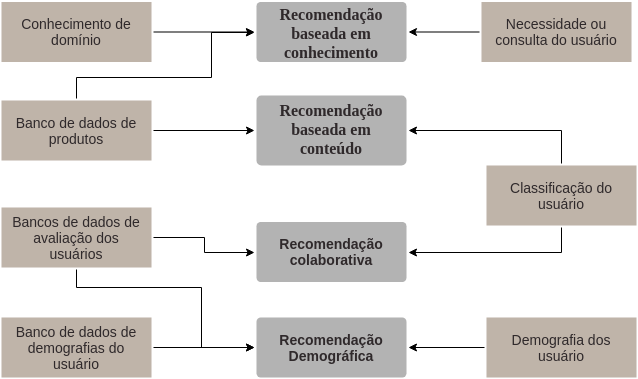
\includegraphics[width=.8\textwidth]{figuras/secao-referencial/tecnicasRecomendacao.png}
\caption{Técnicas de Recomendação e fontes de conhecimento. Adaptado de \cite{burke2007hybrid}.}
\label{img:recomendacao}
\end{figure}

